\section{Additional Tables and Figures}\label[appendix]{app:tables}

\begin{table}[h]
\centering\small
\caption{Accuracy first, then what each answer costs. Bold marks the highest point estimate per model; where the
95\% intervals overlap, the difference is not significant (see the McNemar $p$ values in \cref{tab:accuracy}).
Context = median input tokens per question read by the agent model, and in \CC{} separately by the broker's planner
(\code{llama-3.3-70b}); output = median output tokens of the agent model. Cost is the mean USD per question
(provider-reported for frontier models, Workers AI list prices for open-weight models, planner included in \CC{});
cost per correct answer is total cost divided by correct answers.}
\label{tab:usage}
\setlength{\tabcolsep}{3pt}\footnotesize
\begin{tabular}{@{}l c c r r r r r@{}}
\toprule
 & & & \multicolumn{2}{c}{Context (input tokens)} & & \multicolumn{2}{c}{Cost (USD)}\\
\cmidrule(lr){4-5}\cmidrule(lr){7-8}
Agent model & Cond. & Accuracy, \% (95\% interval) & Agent & Planner & Output & per question & per correct\\
\midrule
\inputtab{tables/tab_usage.tex}
\bottomrule
\end{tabular}
\end{table}

\begin{figure}[h]
\centering
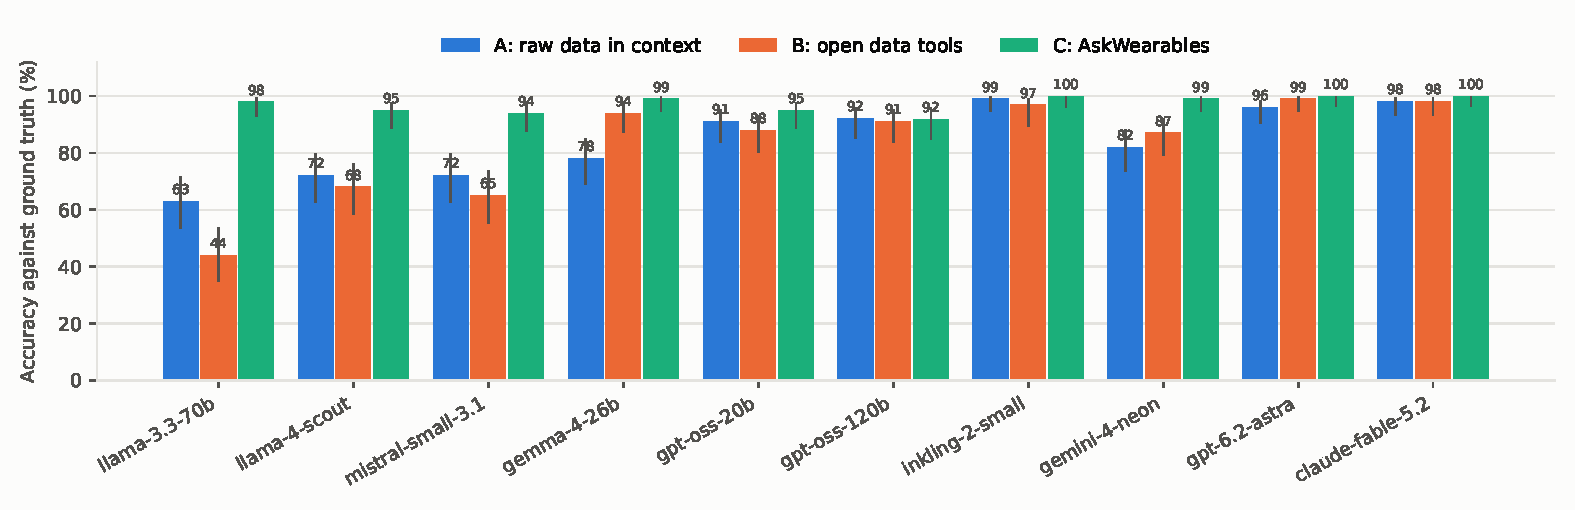
\includegraphics[width=\textwidth]{figures/fig_accuracy.pdf}
\caption{Accuracy against ground truth by model and condition, with Wilson 95\% intervals (the data of
\cref{tab:accuracy}).}
\label{fig:accuracy}
\end{figure}

\begin{table}[h]
\centering\small
\caption{Step~1 against the study's \sys{} on the same tasks, per model (condition \CC{} only): the synthetic
questions, and real data for the open-weight models. Accuracy in \%; \CC{}$_1$-only and \CC{}-only count tasks
right only after step~1 or only in the study; $p$ is the exact McNemar test.}
\label{tab:v2reg}
\setlength{\tabcolsep}{4pt}\footnotesize
\begin{tabular}{@{}l r c c r r c@{}}
\toprule
Agent model & tasks & \CC{} & \CC{}$_1$ & \CC{}$_1$-only & \CC{}-only & $p$\\
\midrule
\multicolumn{7}{@{}l}{\emph{Synthetic questions}}\\
\inputtab{tables/tab_v2_accuracy.tex}
\midrule
\multicolumn{7}{@{}l}{\emph{Real data}}\\
\inputtab{tables/tab_v2_real.tex}
\bottomrule
\end{tabular}
\end{table}

\section{Reproducibility Notes}\label[appendix]{app:repro}

\paragraph{Harness.} Tool-call arguments that are not valid JSON are passed to the tool as an empty object, and the
tool result says so. The planner in the study was called without schema-constrained decoding, and its JSON was
validated afterwards.

\paragraph{Deployed broker.} Besides the two steps of \cref{sec:res:v2}, the deployed broker requests
schema-constrained decoding from the model provider, and it drops the keyword pre-check for sensitive categories:
the planner prompt and the code check on the plan refuse them (all 20 sensitive test questions and none of 10
near-misses were refused without the pre-check).
